\documentclass[11pt,a4paper]{article}

\usepackage[utf8]{inputenc}
\usepackage{amsmath}
\usepackage{amsfonts}
\usepackage{amssymb}
\usepackage{parskip} 
\usepackage[left=1.5cm,right=1.5cm,top= 1.5cm,bottom=1.5cm]{geometry}
\usepackage{graphicx}
\usepackage{float}
\usepackage{subcaption} 
\usepackage{multicol}

\usepackage{Sweave}
\begin{document}
\Sconcordance{concordance:SemiMarkov_Paper.tex:SemiMarkov_Paper.Rnw:%
1 13 1 1 0 4 1 1 6 1 1 1 12 38 1 1 2 11 0 1 2 4 1 1 4 7 0 1 2 9 1 1 33 %
6 1 1 8 5 0 1 2 19 0 1 2 3 1 1 5 5 0 1 2 17 0 1 3 2 1 1 5 5 0 1 2 35 0 %
1 2 8 1 1 7 2 1 1 5 5 0 1 1 15 0 1 3 49 0 1 4 53 0 1 2 2 1 1 4 1 2 3 1 %
1 5 10 0 1 2 6 1 1 5 5 0 1 1 15 0 1 3 49 0 1 4 53 0 1 2 2 1 1 5 1 2 3 1 %
1 6 10 0 1 2 6 1 1 5 5 0 1 1 15 0 1 3 49 0 1 4 53 0 1 2 2 1 1 5 1 2 3 1 %
1 6 10 0 1 2 6 1 1 5 5 0 1 1 15 0 1 3 49 0 1 4 53 0 1 2 2 1 1 5 1 2 3 1 %
1 6 10 0 1 2 10 1 1 5 5 0 1 1 51 0 1 3 42 0 1 3 53 0 1 2 30 1}

  	

%create global options for evaluating all R codes in my document

% load required packages

\newpage

\begin{abstract}
\noindent\textbf{Abstract}—The purpose of this study is to model the transitions of HIV viral load of patients under differentiated care using homogeneous semi-Markov processes. The model focuses on the patient’s WHO staging and DCM as factors. A sample of 366 patients ordered chronologically  was taken from a hospital record in Kenya.  A total of 918 states were observed where 39.87\% and 60.13\% are in similar and different states respectively. The states of viral load were defined based on the WHO HIV staging classification of HIV/AIDS infected patients, we picked 3 states viral loads as follows: <400(stage 1); 400 to 600 (stage 2); 600 to 999 (stage 3). The three states are living states. We assume the living states communicate with each other. We don’t have the absorbing states.\\

\textbf{Keywords:} disease transition, homogeneous semi-Markov process, HIV/AIDS

\end{abstract}


\section{Introduction}
For more than four decades now, human immunodeficiency virus (HIV) infection has become the epicentre of the diseases challenging humanity and a major focus of public health specialists and researchers. Laboratory measurement of plasma HIV viral load is used to determine the extent of body immune destruction as well as monitor the disease progression. The World Health Organization (WHO) has put in place clinical staging that uses various clinical parametres to aid in managing the HIV patients. The WHO staging puts both adults and children into 4 hierarchical stages ;stage 1(asymptomatic) to stage 4 (AIDS) depending on viral load suppression and various observable clinical conditions.\\

The purpose of this study is
\begin{enumerate}
    \item[(a.)] What is the effects of putting patients under differentiated care(DCM) on their viral load?
    \item[(b.)] To model the transition states of HIV viral load of patients under DCM
    \item[(b.)] To determine and select the appropriate distributions which describes the various transition states.

\end{enumerate}


\section{Literature Overview}
\begin{multicols}{2}
In most longitudinal medical studies on the progression of healthy individuals to chronic diseases, the natural development is often expressed in terms of distinct states. The analyses in such studies where individuals may transition among several states are performed by using multi-state models which can either be discrete or continuous. Multi-state models based on the discrete-time Markov chain have become popular in analyzing longitudinal data collected in chronic disease studies. Such models are also called Markov chain transitional models (Agresti 2002). Kryscio, Schmitt, and Salazar (2006) used a Markov chain model to identify risk factors
associated with transitions from cognitively normal to various forms of mild cognitive impairment (MCI) and then from MCI into early dementia, with death before dementia as a competing state. A continuous-time MSM is a model for a continuous time stochastic process allowing individuals to move among a finite number of states (Meira-Machado et al. (2009). There exists an extensive literature on continuous-time MSMs (see, e.g., Hougard (1999) or Commenges (1999))., Hubbard and Zhou (2011), or Joly, Commenges, and Letenneur (1998), Joly, and Commenges (1999), Joly et al. (2002). Applications of continuous-time MSMs can be found in liver cirrhosis (Andersen, Esbjerg, and Sorensen (2000)), dementia (Joly, Commenges, and Letenneur 1998, Joly, and Commenges 1999, Joly et al. 2002; Hubbard and Zhou 2011) among others.
The use of multi-state Markov models to analyze the factors associated with transitions between different states of chronicity has been suggested for chronic diseases and the cost-effectiveness of various therapeutic regimes (Shih et al., 2007; Pan et al., 2007; Gil et al., 2007). Recent studies have shown that the predicted probability of patients that changing their status given
his/her current status allows the measurements of medical scientific progresses due to the advances in the treatment of the HIV/AIDS (D'Amico et al., 2009). Masala et al. (2014; Goshu and Dessie, 2013; Giuseppe et al., 2007) analyzed HIV/AIDS dynamic evolution as defined by CD4 levels from a macroscopic point of view by means of homogeneous semi-Markov stochastic processes Numerical analyses of the homogeneous semi-Markov process are dealt by
Corradi et al. (2004; Janssen and Manca, 2001). Other more readings include (Davidov and Zelen, 2000; Viladent and Van Ackere, 2007; Satten and Sternberg, 1999; Baryarama et al., 2005). In this study, the author, a procedure to obtain the parameters in a model with covariates has been reported (Maciulis et al., 2009; Gentlemann et al.,1985; Mathieu et al., 2007; P<U+0450>rez-Oc<U+03CC>n et al., 2001).
\end{multicols}

\section{Data Exploration and Analysis}
  \subsection{Data Description}
WHO staging (0 for any staging greater than 1 i.e. 2,3 and 4. and 1 for stage 1), DCM(yes= 1, No= 0), AgeGroup(adult= 1, child= 0) and Sex(Female= 1, Male= 0)  \\
A total of 552 different transitions states and 366 HIV patients was studied as shown in the table below.


\begin{minipage}{0.45\textwidth}
\begin{Schunk}
\begin{Soutput}
$table.state
    1   2   3
1 151  94  43
2 112 115  70
3 114 119 100

$Ncens
[1] 366
\end{Soutput}
\end{Schunk}
\end{minipage}%
\hfill
\begin{minipage}{0.45\textwidth}
\begin{tabular}{|p{\textwidth}}
Transition probability matrix
\begin{Schunk}
\begin{Soutput}
            1         2         3
  1 0.5243056 0.3263889 0.1493056
  2 0.3771044 0.3872054 0.2356902
  3 0.3423423 0.3573574 0.3003003
\end{Soutput}
\end{Schunk}
\end{tabular}
\end{minipage}%
\\

The probability of transitioning from a lower state to a higher state is lower than the vice versa. There is a high probability of patient remaining in the same state, more illustrated by 1-->1 transition.\\

Drawing of HIV transition states\\
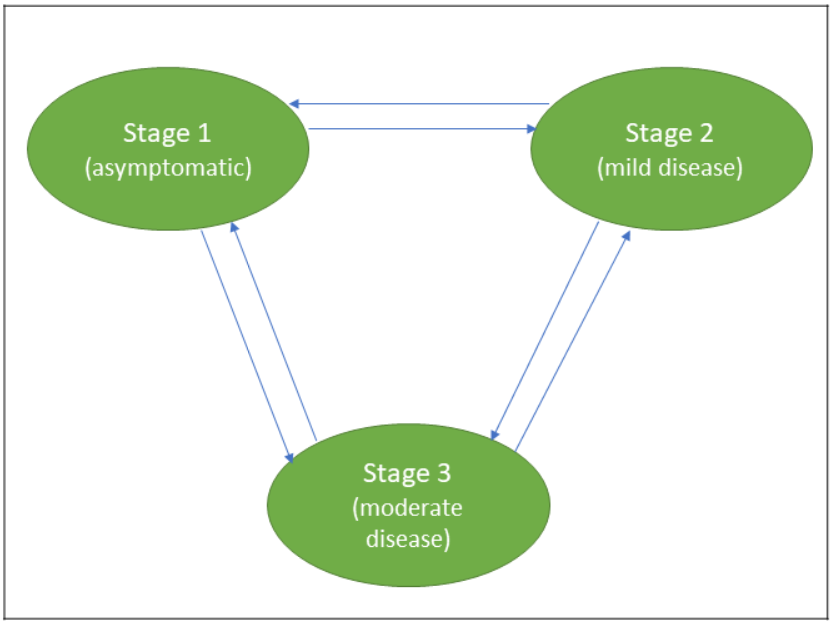
\includegraphics[scale=0.2]{diagram2.PNG}




\subsection{Model Fitting and Selection}
  
\textbf{Weibull distribution}\\

The transitions between the different states are significant since all the p-values < 10\%, at \(\alpha\) = 10\%.
\begin{Schunk}
\begin{Soutput}
Iter: 1 fn: 1615.2486	 Pars:  9.36243 2.94492 6.63966 3.06917 2.43166 5.72270 1.35845 3.90000 1.41184 3.58816 7.68670 1.61996 0.83719 0.73928 0.34749
Iter: 2 fn: 1615.2486	 Pars:  9.36258 2.94492 6.63965 3.06917 2.43166 5.72268 1.35843 3.90001 1.41184 3.58815 7.68668 1.61996 0.83719 0.73928 0.34749
solnp--> Completed in 2 iterations
\end{Soutput}
\begin{Soutput}
$Sigma
  Type Index Transition Sigma   SD Lower_CI Upper_CI Wald_H0 Wald_test p_value
1 dist     1     1 -> 2 9.363 0.84     7.72    11.01    1.00     99.16 <0.0001
2 dist     2     1 -> 3 2.945 0.13     2.70     3.19    1.00    236.13 <0.0001
3 dist     3     2 -> 1  6.64 0.47     5.72     7.56    1.00    143.66 <0.0001
4 dist     4     2 -> 3 3.069 0.11     2.85     3.29    1.00    335.01 <0.0001
5 dist     5     3 -> 1 2.432 0.03     2.37     2.49    1.00   2049.64 <0.0001
6 dist     6     3 -> 2 5.723 0.34     5.06     6.38    1.00    197.66 <0.0001

$Nu
  Type Index Transition    Nu   SD Lower_CI Upper_CI Wald_H0 Wald_test p_value
1 dist     7     1 -> 2 1.358 0.12     1.12     1.59    1.00      8.91  0.0028
2 dist     8     1 -> 3   3.9 0.41     3.09     4.71    1.00     49.17 <0.0001
3 dist     9     2 -> 1 1.412 0.11     1.20     1.63    1.00     14.09  0.0002
4 dist    10     2 -> 3 3.588 0.29     3.02     4.16    1.00     79.49 <0.0001
5 dist    11     3 -> 1 7.687 0.44     6.83     8.55    1.00    233.01 <0.0001
6 dist    12     3 -> 2  1.62 0.12     1.38     1.86    1.00     26.33 <0.0001
\end{Soutput}
\end{Schunk}

\textbf{Exponential distribution}

The p-value for transition between 1-->3 is \textbf{0.1726} which is greater than  =10\%.This transition under exponential is insignificant. 
\begin{Schunk}
\begin{Soutput}
Iter: 1 fn: 1894.9202	 Pars:  9.66638 6.90269 5.00360 7.24220 3.99801 5.19016 0.73265 0.56477 0.45916
Iter: 2 fn: 1894.9202	 Pars:  9.66675 6.90192 5.00366 7.24206 3.99801 5.19017 0.73267 0.56478 0.45916
solnp--> Completed in 2 iterations
\end{Soutput}
\begin{Soutput}
$Sigma
  Type Index Transition Estimation   SD Lower_CI Upper_CI Wald_H0 Wald_test
1 dist     1     1 -> 2      9.667 2.16     5.43    13.91    1.00     16.04
2 dist     2     1 -> 3      6.902 4.33    -1.58    15.38    1.00      1.86
3 dist     3     2 -> 1      5.004 1.09     2.88     7.13    1.00     13.60
4 dist     4     2 -> 3      7.242 1.79     3.74    10.74    1.00     12.20
5 dist     5     3 -> 1      3.998 0.66     2.70     5.29    1.00     20.57
6 dist     6     3 -> 2       5.19 0.71     3.81     6.57    1.00     35.21
  p_value
1  0.0001
2  0.1726
3  0.0002
4  0.0005
5 <0.0001
6 <0.0001
\end{Soutput}
\end{Schunk}

\textbf{Exponentiated weibull distribution}
The p-value for transition between 1-->3 is \textbf{0.729} which is greater than  10\%.This transition under exponential-weibul is insignificant.\\
\begin{Schunk}
\begin{Soutput}
Iter: 1 fn: 1422.7852	 Pars:     0.001000    0.346838    0.001163    0.252479    0.884566    0.001862    0.203835    0.959422    0.229578    0.835604    2.085512    0.253494  272.830439  596.862229  530.652773  807.162884  999.999241  764.772300    0.839091    0.742389    0.346547
Iter: 2 fn: 1422.7851	 Pars:     0.001000    0.346838    0.001163    0.252479    0.884566    0.001862    0.203835    0.959422    0.229578    0.835604    2.085511    0.253494  272.830771  596.862829  530.653458  807.163023  999.999241  764.772776    0.839091    0.742389    0.346548
solnp--> Completed in 2 iterations
\end{Soutput}
\begin{Soutput}
$Sigma
  Type Index Transition Sigma   SD Lower_CI Upper_CI Wald_H0 Wald_test p_value
1 dist     1     1 -> 2 0.001 0.00     0.00     0.00    1.00       Inf <0.0001
2 dist     2     1 -> 3 0.347 0.08     0.19     0.50    1.00     65.84 <0.0001
3 dist     3     2 -> 1 0.001 0.00     0.00     0.00    1.00       Inf <0.0001
4 dist     4     2 -> 3 0.252 0.05     0.15     0.36    1.00    190.71 <0.0001
5 dist     5     3 -> 1 0.885 0.06     0.77     1.00    1.00      4.05  0.0442
6 dist     6     3 -> 2 0.002 0.00     0.00     0.00    1.00       Inf <0.0001

$Nu
  Type Index Transition    Nu   SD Lower_CI Upper_CI Wald_H0 Wald_test p_value
1 dist     7     1 -> 2 0.204 0.02     0.17     0.24    1.00   1920.84 <0.0001
2 dist     8     1 -> 3 0.959 0.12     0.73     1.19    1.00      0.12  0.7290
3 dist     9     2 -> 1  0.23 0.02     0.20     0.26    1.00   1914.68 <0.0001
4 dist    10     2 -> 3 0.836 0.08     0.68     0.99    1.00      4.30  0.0381
5 dist    11     3 -> 1 2.086 0.15     1.80     2.37    1.00     55.50 <0.0001
6 dist    12     3 -> 2 0.253 0.02     0.22     0.29    1.00   1547.98 <0.0001

$Theta
  Type Index Transition   Theta   SD Lower_CI Upper_CI Wald_H0 Wald_test
1 dist    13     1 -> 2 272.831 0.00   272.83   272.83    1.00       Inf
2 dist    14     1 -> 3 596.863 0.00   596.86   596.86    1.00       Inf
3 dist    15     2 -> 1 530.653 0.00   530.65   530.65    1.00       Inf
4 dist    16     2 -> 3 807.163 0.00   807.16   807.16    1.00       Inf
5 dist    17     3 -> 1 999.999 0.00  1000.00  1000.00    1.00       Inf
6 dist    18     3 -> 2 764.773 0.00   764.77   764.77    1.00       Inf
  p_value
1 <0.0001
2 <0.0001
3 <0.0001
4 <0.0001
5 <0.0001
6 <0.0001
\end{Soutput}
\end{Schunk}

We can assume the distribution for all the various transition states follows a Weibull distribution as from the above output. Furthermore, the exponential distribution assumes constant hazard rate over time, which might not be the case in our case.\\
It is also possible to look closer and tailor a distribution for each transition separately within the transition matrix for optimum results. This is more pronounced for 1-->3 transitions as their p-values differs for Exponential and Exponential-Weibull\\
\newpage
\subsubsection{Covariates}

All our covariates are time fixed, hence we are going to use \textbf{"Model-fit-1"} to estimate hazard rates of covariates for both sojourn time and hazard rate due to semi-Markov process.\\

\textbf{Models with select covariates}

\begin{enumerate}
  \item[1] \textbf{WHOStaging}
\begin{Schunk}
\begin{Soutput}
Iter: 1 fn: 1570.7514	 Pars:   8.84188  3.02581  2.61425  6.03014  2.43860  6.45699  1.35784  3.93035  3.65024  1.44291  7.68122  1.63698  0.83778  0.40671  0.34757 -0.09380  0.18117 -0.23733 -0.82106  0.03216  0.35253
Iter: 2 fn: 1570.7514	 Pars:   8.84180  3.02581  2.61425  6.03012  2.43860  6.45699  1.35784  3.93032  3.65024  1.44291  7.68126  1.63699  0.83778  0.40671  0.34757 -0.09382  0.18116 -0.23732 -0.82106  0.03216  0.35253
solnp--> Completed in 2 iterations
\end{Soutput}
\begin{Soutput}
  Type Index Transition Covariates  Estimation   SD Lower_CI Upper_CI Wald_H0
1 coef     1     1 -> 2      Beta1 -0.09381620 0.27    -0.63     0.44    0.00
2 coef     2     1 -> 3      Beta1  0.18115586 0.33    -0.47     0.83    0.00
3 coef     3     2 -> 1      Beta1 -0.23732091 0.28    -0.80     0.32    0.00
4 coef     4     2 -> 3      Beta1 -0.82105857 0.24    -1.29    -0.35    0.00
5 coef     5     3 -> 1      Beta1  0.03215509 0.21    -0.37     0.43    0.00
6 coef     6     3 -> 2      Beta1  0.35252742 0.19    -0.02     0.72    0.00
  Wald_test p_value
1      0.12  0.7290
2      0.30  0.5839
3      0.70  0.4028
4     11.65  0.0006
5      0.02  0.8875
6      3.49  0.0617
\end{Soutput}
\begin{Soutput}
model_fit_1a  : Hazard rates of waiting times

Transition_matrix
  1         2         3        
1 "-"       "Weibull" "Weibull"
2 "Weibull" "-"       "Weibull"
3 "Weibull" "Weibull" "-"      

Hazard rates values 
          12           13           21          23           31         32
1 0.01140972 4.415293e-08 2.422551e-07 0.005609586 8.514372e-17 0.00509113
2 0.01462161 3.365698e-07 1.520804e-06 0.007625362 8.737985e-15 0.00791710
3 0.01690470 1.104281e-06 4.454064e-06 0.009125429 1.311965e-13 0.01025024
4 0.01873766 2.565611e-06 9.547144e-06 0.010365496 8.967470e-13 0.01231170
5 0.02029520 4.933654e-06 1.724677e-05 0.011442282 3.982452e-12 0.01419216
6 0.02166345 8.417739e-06 2.796126e-05 0.012404605 1.346421e-11 0.01593991

     Time
1 0.00804
2 0.01608
3 0.02412
4 0.03216
5 0.04020
6 0.04824

  cova
1    1
2    1
3    1
4    1
5    1
6    1

Summary statistics
                12           13           21          23           31
Min.    0.01140972 4.415293e-08 2.422551e-07 0.005609586 8.514372e-17
1st Qu. 0.08237883 4.737165e-01 5.531317e-01 0.064801047 9.122660e-01
Median  0.10549348 3.589977e+00 3.454058e+00 0.088009150 9.237877e+01
Mean    0.09959187 6.955986e+00 5.935399e+00 0.082933896 1.230713e+03
3rd Qu. 0.12193668 1.175567e+01 1.009823e+01 0.105291316 1.380844e+03
Max.    0.13514204 2.728564e+01 2.162612e+01 0.119581849 9.417214e+03
                32
Min.    0.00509113
1st Qu. 0.17182949
Median  0.26686869
Mean    0.25356076
3rd Qu. 0.34536719
Max.    0.41473737
\end{Soutput}
\begin{Soutput}
[1] "1 1 0 1 6 6 7.16265058538368e-09 0.999943402590078"
[1] "2 2 0 1 6 6 0.00332798845823161 0.999981455717204"
[1] "3 3 0 1 6 6 0.00332153830189253 0.999983686179198"
model_fit_1a  : Hazard rates of the semi-Markov process

Transition_matrix
  1         2         3        
1 "-"       "Weibull" "Weibull"
2 "Weibull" "-"       "Weibull"
3 "Weibull" "Weibull" "-"      

Hazard rates values 
           12           13           21          23           31          32
1 0.009558691 7.163056e-09 9.853020e-08 0.003328050 2.959362e-17 0.003321592
2 0.012249295 5.460752e-08 6.185624e-07 0.004523869 3.037188e-15 0.005165239
3 0.014161666 1.791857e-07 1.811691e-06 0.005413659 4.560405e-14 0.006687242
4 0.015696836 4.163577e-07 3.883483e-06 0.006149133 3.117288e-13 0.008031887
5 0.017001184 8.007585e-07 7.015818e-06 0.006787674 1.384483e-12 0.009258313
6 0.018146855 1.366437e-06 1.137501e-05 0.007358246 4.681147e-12 0.010398027

     Time
1 0.00804
2 0.01608
3 0.02412
4 0.03216
5 0.04020
6 0.04824

  cova
1    1
2    1
3    1
4    1
5    1
6    1

Summary statistics
                 12           13           21         23            31
Min.    0.009558691 6.756099e-24 5.934125e-20 0.00332805 1.725771e-320
1st Qu. 0.070311728 5.227794e-08 5.636767e-07 0.04172830 3.633853e-320
Median  0.104790662 2.474467e-03 8.752045e-03 0.08632987  9.711059e-20
Mean    0.095496476 2.611133e-02 7.272784e-02 0.07514161  6.648766e-02
3rd Qu. 0.121936676 4.711874e-02 1.343554e-01 0.10529131  7.871063e-03
Max.    0.135142038 1.095453e-01 2.952731e-01 0.11958185  6.602145e-01
                 32
Min.    0.003321592
1st Qu. 0.113186745
Median  0.266868691
Mean    0.240188655
3rd Qu. 0.345367194
Max.    0.414737370
\end{Soutput}
\end{Schunk}

\begin{minipage}{0.45\textwidth}
Sojourn time hazard rate plot for WHOStaging(0,1)\\
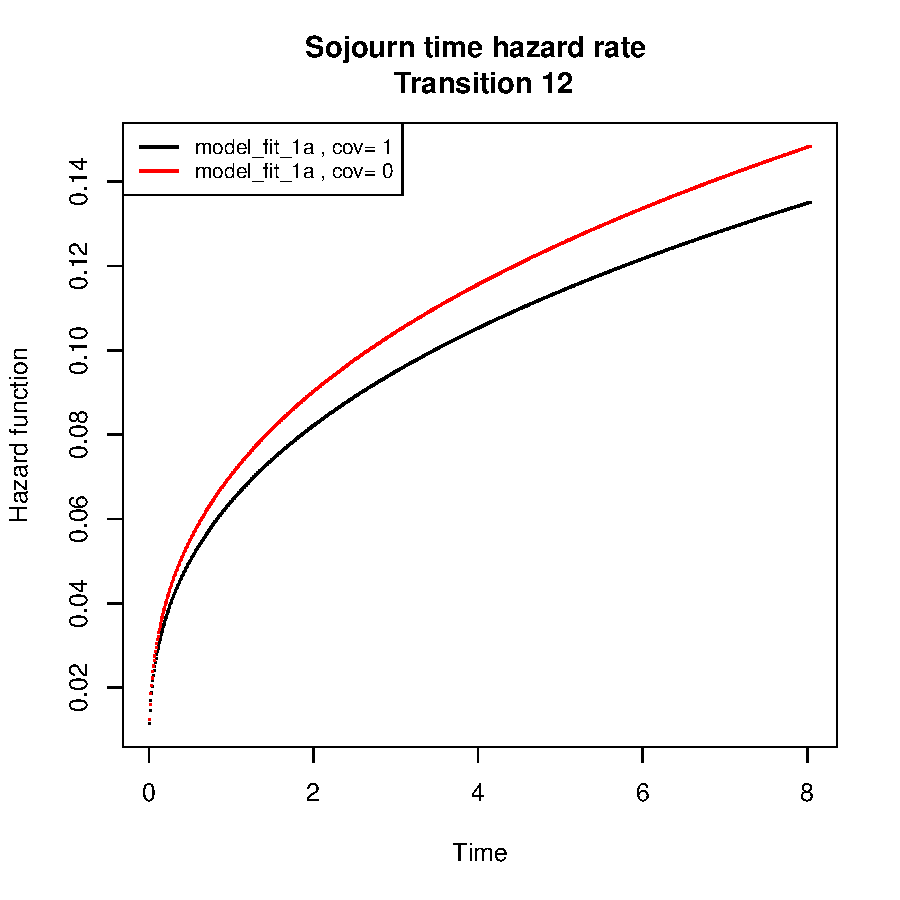
\includegraphics{SemiMarkov_Paper-011}
\end{minipage}%
\begin{minipage}{0.45\textwidth}
\begin{tabular}{|p{\textwidth}}
Semi-Markov process hazard rate plot for WHOStaging\\
\begin{Schunk}
\begin{Soutput}
[1] "1 1 0 1 6 6 7.16265058538368e-09 0.999943402590078"
[1] "2 2 0 1 6 6 0.00332798845823161 0.999981455717204"
[1] "3 3 0 1 6 6 0.00332153830189253 0.999983686179198"
[1] "1 1 0 1 6 6 5.97583741651534e-09 0.999937836000994"
[1] "2 2 0 1 6 6 0.00756389933358081 0.999957851670866"
[1] "3 3 0 1 6 6 0.00233475749879611 0.999988532821086"
\end{Soutput}
\end{Schunk}
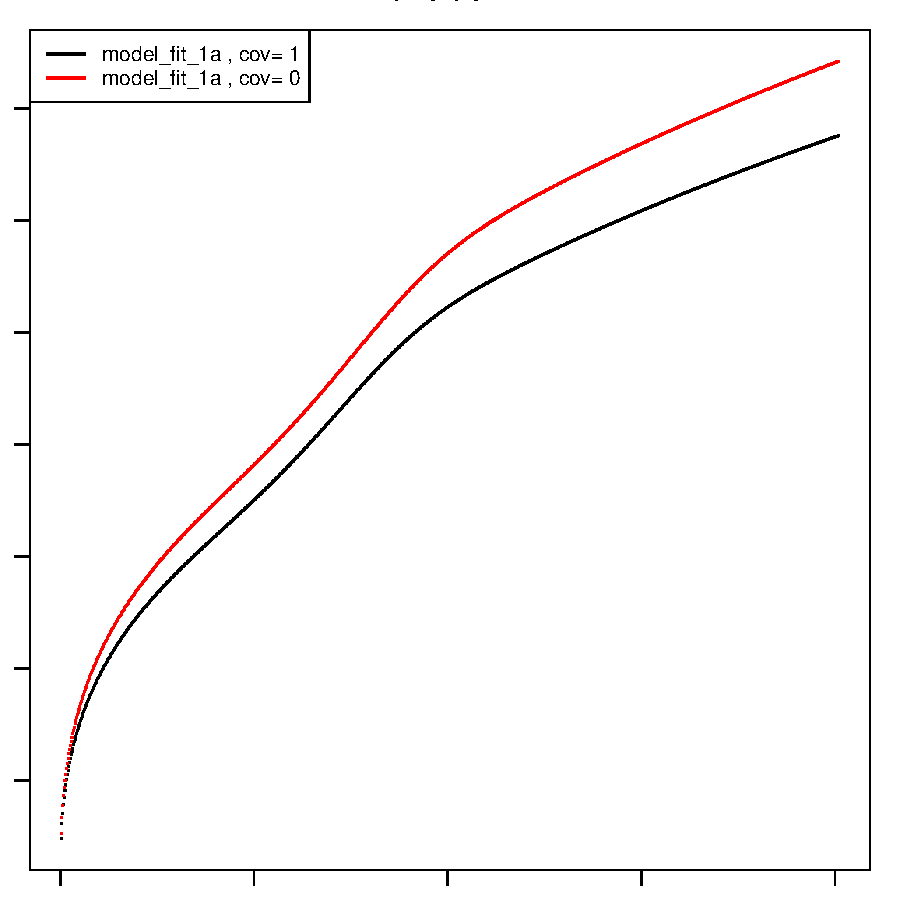
\includegraphics{SemiMarkov_Paper-012}
\end{tabular}
\end{minipage}%
\end{enumerate}

WHOStaging as a variables has no cause-effect relationship on HIV patient transition states.We drop this variable from our model.\\
\begin{enumerate}
  \item[2] \textbf{DCM}
\begin{Schunk}
\begin{Soutput}
Iter: 1 fn: 1715.2221	 Pars:   8.71362  2.51413  6.79600  2.98071  2.33683  5.23252  1.35909  4.78302  1.41417  3.63128  2.90509  2.02684  0.83860  0.73864  0.48210 -0.29699 -1.29338  0.08715 -0.24765 -2.82641  0.99435
Iter: 2 fn: 1715.2221	 Pars:   8.71356  2.51412  6.79611  2.98069  2.33681  5.23251  1.35911  4.78311  1.41416  3.63130  2.90516  2.02683  0.83860  0.73864  0.48210 -0.29700 -1.29343  0.08715 -0.24768 -2.82645  0.99426
solnp--> Completed in 2 iterations
\end{Soutput}
\begin{Soutput}
  Type Index Transition Covariates  Estimation   SD Lower_CI Upper_CI Wald_H0
1 coef     1     1 -> 2      Beta1 -0.29700347 0.23    -0.74     0.15    0.00
2 coef     2     1 -> 3      Beta1 -1.29342573 0.39    -2.06    -0.52    0.00
3 coef     3     2 -> 1      Beta1  0.08715437 0.19    -0.29     0.47    0.00
4 coef     4     2 -> 3      Beta1 -0.24768095 0.26    -0.76     0.26    0.00
5 coef     5     3 -> 1      Beta1 -2.82644619 0.32    -3.45    -2.20    0.00
6 coef     6     3 -> 2      Beta1  0.99425582 0.29     0.43     1.56    0.00
  Wald_test p_value
1      1.73  0.1884
2     10.80  0.0010
3      0.20  0.6547
4      0.90  0.3428
5     77.99 <0.0001
6     12.04  0.0005
\end{Soutput}
\begin{Soutput}
model_fit_1b  : Hazard rates of waiting times

Transition_matrix
  1         2         3        
1 "-"       "Weibull" "Weibull"
2 "Weibull" "-"       "Weibull"
3 "Weibull" "Weibull" "-"      

Hazard rates values 
           12           13         21           23           31          32
1 0.009423116 1.897786e-10 0.01392639 1.652741e-07 1.492567e-06 0.001351977
2 0.012086414 2.612619e-09 0.01855724 1.024013e-06 5.590403e-06 0.002754710
3 0.013980852 1.211291e-08 0.02195045 2.976150e-06 1.210388e-05 0.004177261
4 0.015502452 3.596708e-08 0.02472795 6.344629e-06 2.093883e-05 0.005612836
5 0.016795842 8.366161e-08 0.02712217 1.141315e-05 3.203179e-05 0.007058176
6 0.017932324 1.667545e-07 0.02924949 1.843977e-05 4.533503e-05 0.008511343

     Time
1 0.00804
2 0.01608
3 0.02412
4 0.03216
5 0.04020
6 0.04824

  cova
1    1
2    1
3    1
4    1
5    1
6    1

Summary statistics
                 12           13         21           23           31
Min.    0.009423116 1.897786e-10 0.01392639 1.652741e-07 1.492567e-06
1st Qu. 0.068515090 2.263820e-01 0.13724924 3.398865e-01 5.557317e-02
Median  0.087816874 3.093050e+00 0.18273674 2.094844e+00 2.073587e-01
Mean    0.082899586 8.889951e+00 0.17223472 3.571372e+00 2.672178e-01
3rd Qu. 0.101557094 1.430418e+01 0.21609075 6.077696e+00 4.483863e-01
Max.    0.112596548 4.242008e+01 0.24340023 1.294522e+01 7.751832e-01
                 32
Min.    0.001351977
1st Qu. 0.393170614
Median  0.799461300
Mean    0.803675826
3rd Qu. 1.211479485
Max.    1.627264818
\end{Soutput}
\begin{Soutput}
[1] "1 1 0 1 6 6 3.06294915976853e-11 0.999953254397904"
[1] "2 2 0 1 6 6 4.31957745364934e-08 0.999941519236846"
[1] "3 3 0 1 6 6 0.000700189376230884 0.999997220499549"
model_fit_1b  : Hazard rates of the semi-Markov process

Transition_matrix
  1         2         3        
1 "-"       "Weibull" "Weibull"
2 "Weibull" "-"       "Weibull"
3 "Weibull" "Weibull" "-"      

Hazard rates values 
           12           13         21           23           31           32
1 0.007902192 3.063092e-11 0.01028640 4.319830e-08 7.195638e-07 0.0007001913
2 0.010135482 4.217168e-10 0.01370639 2.676761e-07 2.695146e-06 0.0014266577
3 0.011723929 1.955381e-09 0.01621193 7.780566e-07 5.835393e-06 0.0021633645
4 0.012999649 5.806727e-09 0.01826241 1.658911e-06 1.009501e-05 0.0029067808
5 0.014083931 1.350827e-08 0.02002953 2.984622e-06 1.544354e-05 0.0036552050
6 0.015036574 2.692786e-08 0.02159926 4.822939e-06 2.185816e-05 0.0044076221

     Time
1 0.00804
2 0.01608
3 0.02412
4 0.03216
5 0.04020
6 0.04824

  cova
1    1
2    1
3    1
4    1
5    1
6    1

Summary statistics
                 12           13        21           23           31
Min.    0.007902192 1.713964e-30 0.0102864 6.519979e-12 7.195638e-07
1st Qu. 0.057399297 3.256393e-08 0.1011932 9.883816e-05 3.166338e-02
Median  0.086221784 1.863885e-03 0.1726526 1.486013e-02 1.603990e-01
Mean    0.078856747 2.593586e-02 0.1583657 5.154933e-02 2.401082e-01
3rd Qu. 0.101557094 4.400595e-02 0.2160828 1.005887e-01 4.174671e-01
Max.    0.112596548 1.157206e-01 0.2434002 1.811436e-01 7.641521e-01
                  32
Min.    0.0007001913
1st Qu. 0.0588202664
Median  0.1192760775
Mean    0.1160804979
3rd Qu. 0.1758142616
Max.    0.1990027585
\end{Soutput}
\end{Schunk}

\begin{minipage}{0.45\textwidth}
Sojourn time hazard rate plot for DCM\\
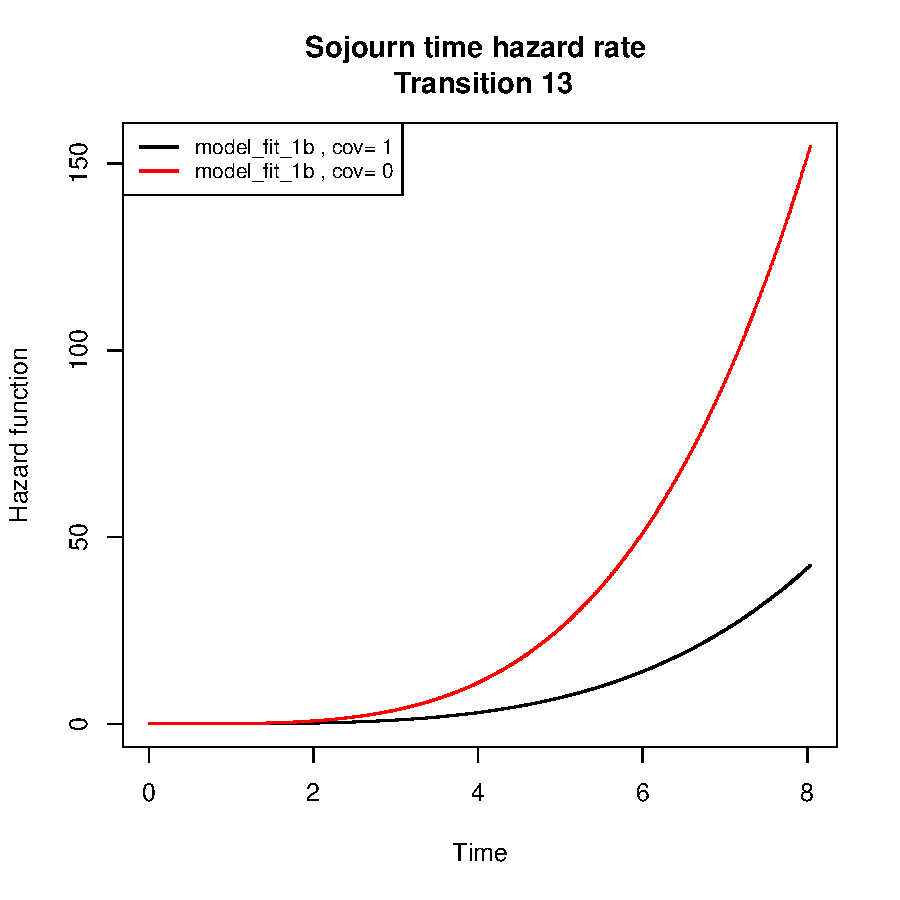
\includegraphics{SemiMarkov_Paper-014}
\end{minipage}%
\begin{minipage}{0.45\textwidth}
\begin{tabular}{|p{\textwidth}}
Semi-Markov process hazard rate plot for DCM\\
\begin{Schunk}
\begin{Soutput}
[1] "1 1 0 1 6 6 3.06294915976853e-11 0.999953254397904"
[1] "2 2 0 1 6 6 4.31957745364934e-08 0.999941519236846"
[1] "3 3 0 1 6 6 0.000700189376230884 0.999997220499549"
[1] "1 1 0 1 6 6 1.11652240850647e-10 0.999937089441428"
[1] "2 2 0 1 6 6 5.53359967007423e-08 0.99994640008663"
[1] "3 3 0 1 6 6 0.000259070025201488 0.999998938698382"
\end{Soutput}
\end{Schunk}
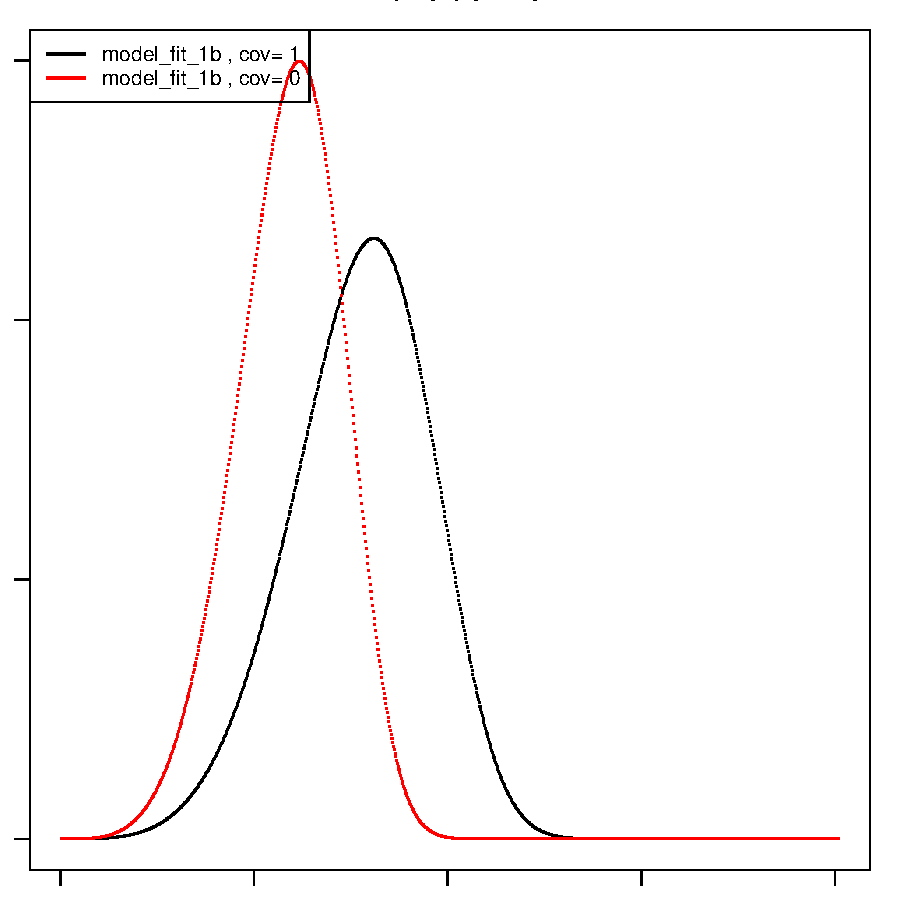
\includegraphics{SemiMarkov_Paper-015}
\end{tabular}
\end{minipage}%
\end{enumerate}

From the two graphs above we can see putting patients under differentiated care model(black line) has a significant impact on their viral load as compared to putting them under zero care (red line). \\The DCM is an important variable to consider in this model.
\begin{enumerate}
  \item[3] \textbf{AgeGroup}
\begin{Schunk}
\begin{Soutput}
Iter: 1 fn: 1675.4531	 Pars:  21.93889  3.33343  2.35866  4.24381  3.67552  2.47044  1.36230  3.94322  3.65736  1.46085  1.51916  3.16851  0.83734  0.40679  0.62510  1.21100  0.55001 -0.60073 -1.09513 -0.72143 -0.56573
Iter: 2 fn: 1675.4531	 Pars:  21.94063  3.33337  2.35855  4.24363  3.67516  2.47044  1.36230  3.94319  3.65737  1.46085  1.51917  3.16855  0.83734  0.40679  0.62510  1.21111  0.54994 -0.60089 -1.09518 -0.72155 -0.56574
solnp--> Completed in 2 iterations
\end{Soutput}
\begin{Soutput}
  Type Index Transition Covariates Estimation   SD Lower_CI Upper_CI Wald_H0
1 coef     1     1 -> 2      Beta1  1.2111096 0.72    -0.19     2.61    0.00
2 coef     2     1 -> 3      Beta1  0.5499446 0.56    -0.54     1.64    0.00
3 coef     3     2 -> 1      Beta1 -0.6008895 0.57    -1.72     0.51    0.00
4 coef     4     2 -> 3      Beta1 -1.0951821 0.44    -1.95    -0.24    0.00
5 coef     5     3 -> 1      Beta1 -0.7215469 0.29    -1.29    -0.16    0.00
6 coef     6     3 -> 2      Beta1 -0.5657355 0.40    -1.34     0.21    0.00
  Wald_test p_value
1      2.87  0.0902
2      0.98  0.3222
3      1.11  0.2921
4      6.31  0.0120
5      6.29  0.0121
6      2.05  0.1522
\end{Soutput}
\begin{Soutput}
model_fit_1c  : Hazard rates of waiting times

Transition_matrix
  1         2         3        
1 "-"       "Weibull" "Weibull"
2 "Weibull" "-"       "Weibull"
3 "Weibull" "Weibull" "-"      

Hazard rates values 
          12           13           21          23          31           32
1 0.01186160 4.051535e-08 2.359397e-07 0.006405906 0.008355284 2.938204e-06
2 0.01524777 3.116082e-07 1.488498e-06 0.008816786 0.011974218 1.320933e-05
3 0.01766054 1.027731e-06 4.372074e-06 0.010628256 0.014779801 3.182318e-05
4 0.01960059 2.396614e-06 9.390650e-06 0.012135007 0.017160626 5.938538e-05
5 0.02125102 4.621925e-06 1.699109e-05 0.013449342 0.019268413 9.634602e-05
6 0.02270215 7.904393e-06 2.758258e-05 0.014628229 0.021181394 1.430679e-04

     Time
1 0.00804
2 0.01608
3 0.02412
4 0.03216
5 0.04020
6 0.04824

  cova
1    1
2    1
3    1
4    1
5    1
6    1

Summary statistics
                12           13           21          23          31
Min.    0.01186160 4.051535e-08 2.359397e-07 0.006405906 0.008355284
1st Qu. 0.08777821 4.667143e-01 5.603619e-01 0.081709247 0.147087812
Median  0.11275499 3.568507e+00 3.516499e+00 0.112357373 0.210577861
Mean    0.10642703 6.953521e+00 6.060781e+00 0.105885604 0.198697726
3rd Qu. 0.13056559 1.174639e+01 1.031051e+01 0.135400409 0.259826807
Max.    0.14489105 2.736509e+01 2.212602e+01 0.154572183 0.301629187
                  32
Min.    2.938204e-06
1st Qu. 4.687693e-01
Median  2.098346e+00
Mean    2.975507e+00
3rd Qu. 5.047915e+00
Max.    9.413127e+00
\end{Soutput}
\begin{Soutput}
[1] "1 1 0 1 6 6 6.5900834836288e-09 0.999941384117435"
[1] "2 2 0 1 6 6 0.0037999384636388 0.999979085911323"
[1] "3 3 0 1 6 6 1.10153799402031e-06 0.999972356489069"
model_fit_1c  : Hazard rates of the semi-Markov process

Transition_matrix
  1         2         3        
1 "-"       "Weibull" "Weibull"
2 "Weibull" "-"       "Weibull"
3 "Weibull" "Weibull" "-"      

Hazard rates values 
           12           13           21          23          31           32
1 0.009932121 6.590470e-09 9.597899e-08 0.003800018 0.005222786 1.101568e-06
2 0.012767246 5.069272e-08 6.055352e-07 0.005230034 0.007484706 4.952593e-06
3 0.014787188 1.672108e-07 1.778684e-06 0.006304379 0.009238014 1.193232e-05
4 0.016411196 3.899757e-07 3.820591e-06 0.007197873 0.010725617 2.226873e-05
5 0.017792586 7.521807e-07 6.913254e-06 0.007977137 0.012042353 3.613179e-05
6 0.019007014 1.286566e-06 1.122342e-05 0.008675965 0.013237123 5.365891e-05

     Time
1 0.00804
2 0.01608
3 0.02412
4 0.03216
5 0.04020
6 0.04824

  cova
1    1
2    1
3    1
4    1
5    1
6    1

Summary statistics
                 12           13           21          23          31
Min.    0.009932121 7.327122e-24 2.670350e-20 0.003800018 0.005222786
1st Qu. 0.074753107 5.363924e-08 4.713045e-07 0.052256820 0.095448814
Median  0.111959637 2.532403e-03 8.741631e-03 0.110207016 0.196265137
Mean    0.102008568 2.649868e-02 7.482769e-02 0.096008767 0.179223237
3rd Qu. 0.130565591 4.786671e-02 1.377676e-01 0.135400402 0.259797482
Max.    0.144891047 1.111590e-01 3.052998e-01 0.154572183 0.301629187
                  32
Min.    1.179667e-09
1st Qu. 3.432316e-04
Median  2.888902e-02
Mean    7.791375e-02
3rd Qu. 1.545107e-01
Max.    2.559254e-01
\end{Soutput}
\end{Schunk}

\begin{minipage}{0.45\textwidth}
Sojourn time hazard rate plot for Agegroup\\
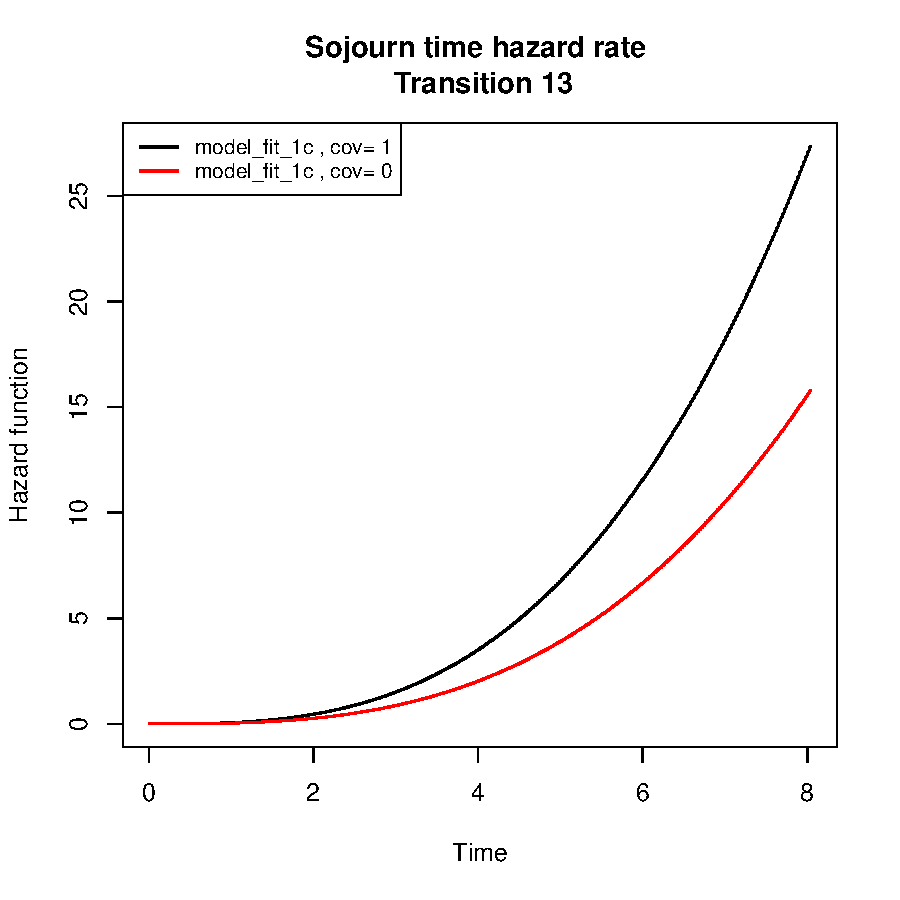
\includegraphics{SemiMarkov_Paper-017}
\end{minipage}%
\begin{minipage}{0.45\textwidth}
\begin{tabular}{|p{\textwidth}}
Semi-Markov process hazard rate plot for Agegroup\\
\begin{Schunk}
\begin{Soutput}
[1] "1 1 0 1 6 6 6.5900834836288e-09 0.999941384117435"
[1] "2 2 0 1 6 6 0.0037999384636388 0.999979085911323"
[1] "3 3 0 1 6 6 1.10153799402031e-06 0.999972356489069"
[1] "1 1 0 1 6 6 3.80235823826545e-09 0.999982539854202"
[1] "2 2 0 1 6 6 0.0113599816666177 0.999937475023631"
[1] "3 3 0 1 6 6 1.93952456710667e-06 0.999943122492991"
\end{Soutput}
\end{Schunk}
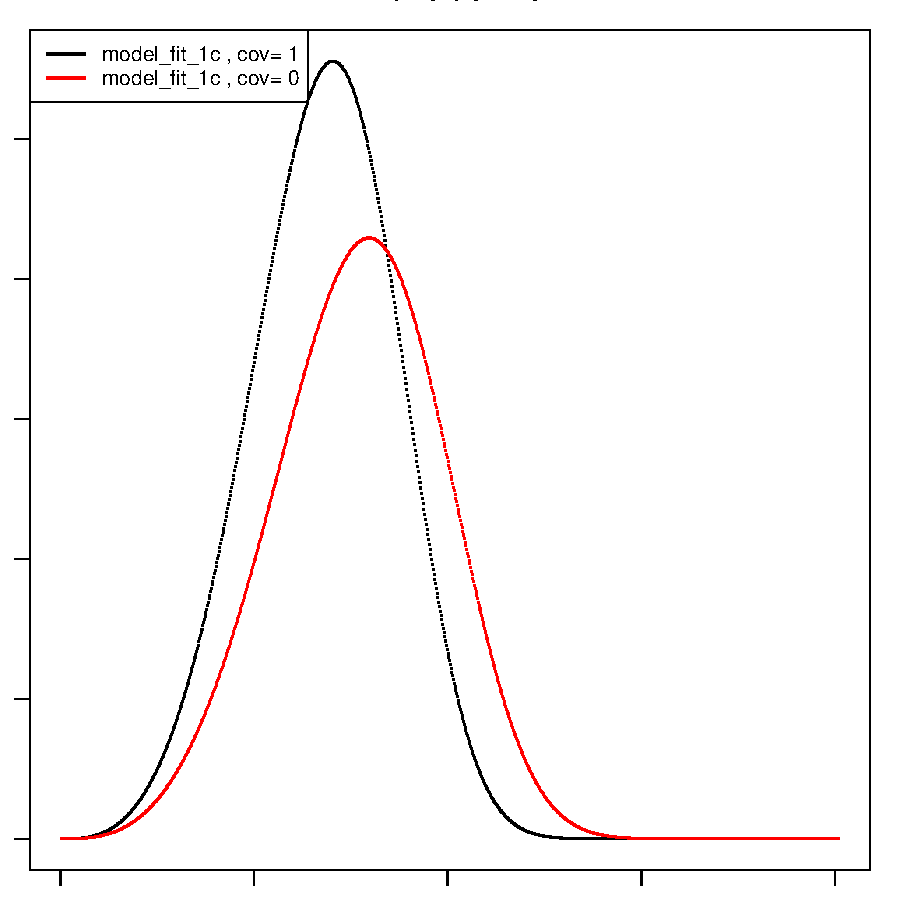
\includegraphics{SemiMarkov_Paper-018}
\end{tabular}
\end{minipage}%
\end{enumerate}

As depicted on the graphs, Adults(black line) can transition to a higher states than children(red line). So the age of patients matters in HIV viral load.\\
\begin{enumerate}
  \item[4] \textbf{Sex}
\begin{Schunk}
\begin{Soutput}
Iter: 1 fn: 1606.7964	 Pars:   8.95237  2.87300  6.96601  3.26589  2.37461  5.19412  1.36046  3.92586  1.41383  3.79177  8.05699  1.64185  0.83723  0.73938  0.34774 -0.14566 -0.21282  0.15657  0.63747 -0.49816 -0.36575
Iter: 2 fn: 1606.7964	 Pars:   8.95231  2.87300  6.96594  3.26589  2.37461  5.19408  1.36046  3.92592  1.41384  3.79178  8.05698  1.64185  0.83723  0.73938  0.34774 -0.14567 -0.21281  0.15655  0.63743 -0.49815 -0.36575
solnp--> Completed in 2 iterations
\end{Soutput}
\begin{Soutput}
  Type Index Transition Covariates Estimation   SD Lower_CI Upper_CI Wald_H0
1 coef     1     1 -> 2      Beta1 -0.1456678 0.21    -0.56     0.27    0.00
2 coef     2     1 -> 3      Beta1 -0.2128112 0.32    -0.85     0.42    0.00
3 coef     3     2 -> 1      Beta1  0.1565528 0.19    -0.22     0.53    0.00
4 coef     4     2 -> 3      Beta1  0.6374350 0.27     0.11     1.17    0.00
5 coef     5     3 -> 1      Beta1 -0.4981473 0.20    -0.90    -0.10    0.00
6 coef     6     3 -> 2      Beta1 -0.3657513 0.19    -0.74     0.01    0.00
  Wald_test p_value
1      0.48  0.4884
2      0.43  0.5120
3      0.68  0.4096
4      5.60  0.0180
5      5.92  0.0150
6      3.71  0.0541
\end{Soutput}
\begin{Soutput}
model_fit_1d  : Hazard rates of waiting times

Transition_matrix
  1         2         3        
1 "-"       "Weibull" "Weibull"
2 "Weibull" "-"       "Weibull"
3 "Weibull" "Weibull" "-"      

Hazard rates values 
          12           13         21           23           31          32
1 0.01047833 3.741695e-08 0.01444334 1.144546e-07 7.605319e-18 0.003445197
2 0.01345241 2.843537e-07 0.01924178 7.925797e-07 1.012699e-15 0.005375648
3 0.01556945 9.312970e-07 0.02275719 2.458392e-06 1.770734e-14 0.006973574
4 0.01727063 2.160973e-06 0.02563439 5.488487e-06 1.348478e-13 0.008387792
5 0.01871717 4.151456e-06 0.02811435 1.023303e-05 6.512324e-13 0.009679425
6 0.01998856 7.077480e-06 0.03031770 1.702397e-05 2.357852e-12 0.010881085

     Time
1 0.00804
2 0.01608
3 0.02412
4 0.03216
5 0.04020
6 0.04824

  cova
1    1
2    1
3    1
4    1
5    1
6    1

Summary statistics
                12           13         21           23           31
Min.    0.01047833 3.741695e-08 0.01444334 1.144546e-07 7.605319e-18
1st Qu. 0.07675623 3.918006e-01 0.14209049 5.712035e-01 6.494482e-01
Median  0.09847126 2.960170e+00 0.18914031 3.933492e+00 8.526523e+01
Mean    0.09295206 5.724614e+00 0.17827110 7.177197e+00 1.404877e+03
3rd Qu. 0.11394059 9.676063e+00 0.22363393 1.217806e+01 1.483873e+03
Max.    0.12637503 2.243034e+01 0.25187336 2.716283e+01 1.127360e+04
                 32
Min.    0.003445197
1st Qu. 0.119446184
Median  0.186137035
Mean    0.176926132
3rd Qu. 0.241363559
Max.    0.290249202
\end{Soutput}
\begin{Soutput}
[1] "1 1 0 1 6 6 6.09031447106353e-09 0.999948156380348"
[1] "2 2 0 1 6 6 2.98293930982291e-08 0.999939274232146"
[1] "3 3 0 1 6 6 0.00224711061269945 0.99998899601303"
model_fit_1d  : Hazard rates of the semi-Markov process

Transition_matrix
  1         2         3        
1 "-"       "Weibull" "Weibull"
2 "Weibull" "-"       "Weibull"
3 "Weibull" "Weibull" "-"      

Hazard rates values 
           12           13         21           23           31          32
1 0.008772692 6.090630e-09 0.01067886 2.983120e-08 2.644737e-18 0.002247135
2 0.011262485 4.629008e-08 0.01422614 2.065972e-07 3.521728e-16 0.003506232
3 0.013034644 1.516212e-07 0.01682446 6.408951e-07 6.158042e-15 0.004548390
4 0.014458552 3.518593e-07 0.01895062 1.431038e-06 4.689760e-14 0.005470671
5 0.015669185 6.760407e-07 0.02078280 2.668529e-06 2.264975e-13 0.006312938
6 0.016733115 1.152677e-06 0.02241020 4.440215e-06 8.201011e-13 0.007096459

     Time
1 0.00804
2 0.01608
3 0.02412
4 0.03216
5 0.04020
6 0.04824

  cova
1    1
2    1
3    1
4    1
5    1
6    1

Summary statistics
                 12           13         21           23            31
Min.    0.008772692 1.033475e-19 0.01067886 3.888612e-24 1.207991e-320
1st Qu. 0.065150728 7.538733e-07 0.10775889 3.923145e-08 2.031598e-320
Median  0.097253840 3.643321e-03 0.18739923 4.202069e-03  1.237616e-17
Mean    0.088867934 2.618098e-02 0.16698195 4.884554e-02  6.277400e-02
3rd Qu. 0.113940577 4.876009e-02 0.22363393 8.730223e-02  7.281700e-03
Max.    0.126375033 1.045225e-01 0.25187336 2.074295e-01  6.261341e-01
                 32
Min.    0.002247135
1st Qu. 0.078337606
Median  0.186137035
Mean    0.167301448
3rd Qu. 0.241363559
Max.    0.290249202
\end{Soutput}
\end{Schunk}

\begin{minipage}{0.45\textwidth}
Sojourn time hazard rate plot for sex\\
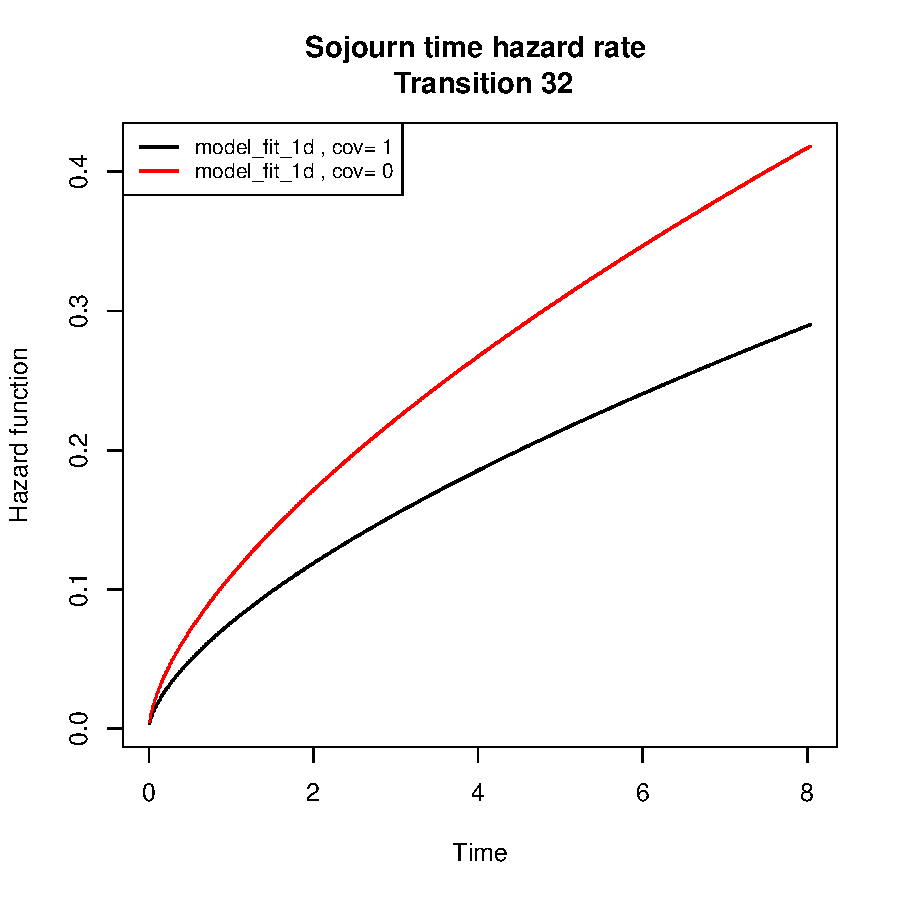
\includegraphics{SemiMarkov_Paper-020}
\end{minipage}%
\begin{minipage}{0.45\textwidth}
\begin{tabular}{|p{\textwidth}}
Semi-Markov process hazard rate plot for Sex\\
\begin{Schunk}
\begin{Soutput}
[1] "1 1 0 1 6 6 6.09031447106353e-09 0.999948156380348"
[1] "2 2 0 1 6 6 2.98293930982291e-08 0.999939274232146"
[1] "3 3 0 1 6 6 0.00224711061269945 0.99998899601303"
[1] "1 1 0 1 6 6 7.5346393434772e-09 0.999940026974986"
[1] "2 2 0 1 6 6 1.57692096921624e-08 0.999948073937727"
[1] "3 3 0 1 6 6 0.00323940293915399 0.999984136748624"
\end{Soutput}
\end{Schunk}
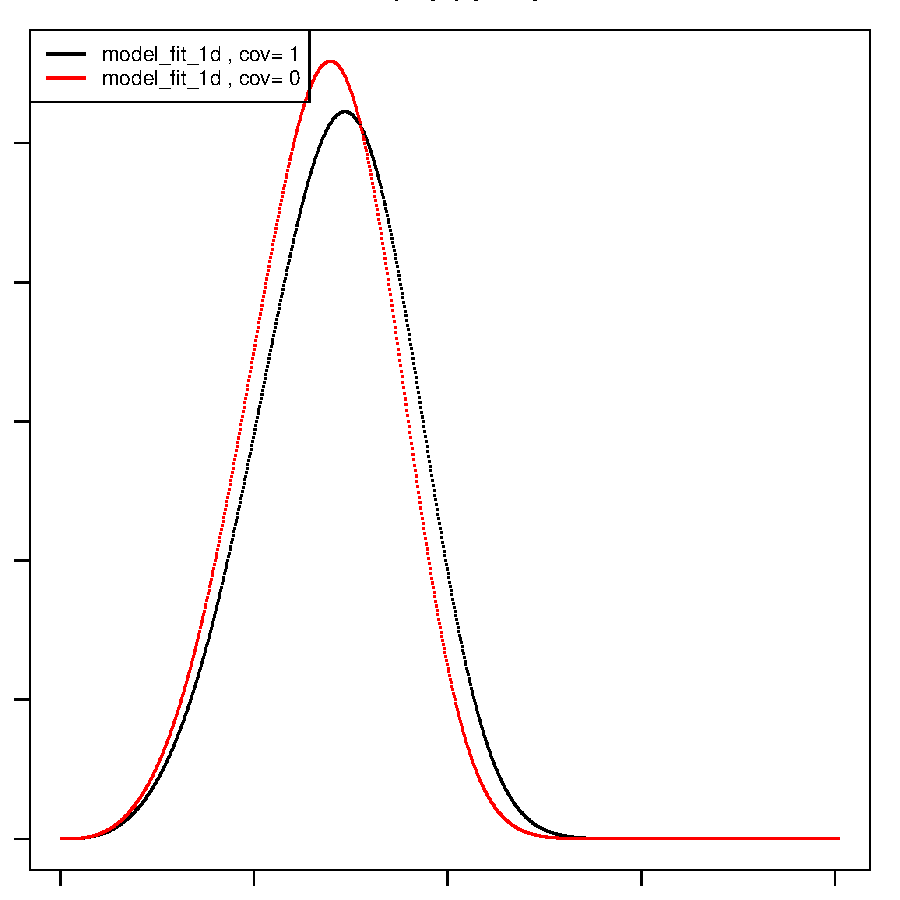
\includegraphics{SemiMarkov_Paper-021}
\end{tabular}
\end{minipage}%
\end{enumerate}

Male(red line) are vulnerable to a higher HIV viral load as compared to female(back line). 


\textbf{Multiple covariate modelling}\\

In combining the covariates, we will need to study the univariate and check which covariate affect what transition and specify in "cov-tra" argument.(Not a final model for now)\\

\begin{Schunk}
\begin{Soutput}
Iter: 1 fn: 1635.6668	 Pars:   2.87154 10.71408  2.21991  4.23328  3.90218  2.24931  3.05315  1.24413  3.70993  1.47196  1.58788  3.43321  0.36763  0.40662  0.62583 -0.36873 -0.91923 -0.22309 -0.74869  0.57206 -0.10327 -0.43752  0.44316 -0.02232  0.15201 -0.51065 -0.05777  0.03737  0.02669 -0.71290 -0.64311 -0.80078 -0.48139  0.31756 -0.20695  0.16510 -0.04056  0.02865 -0.84279
Iter: 2 fn: 1635.6668	 Pars:   2.87158 10.71432  2.21990  4.23326  3.90219  2.24930  3.05314  1.24413  3.70993  1.47196  1.58788  3.43321  0.36763  0.40662  0.62583 -0.36873 -0.91922 -0.22312 -0.74869  0.57206 -0.10327 -0.43752  0.44317 -0.02233  0.15201 -0.51065 -0.05778  0.03742  0.02672 -0.71288 -0.64311 -0.80077 -0.48140  0.31756 -0.20695  0.16510 -0.04056  0.02865 -0.84279
solnp--> Completed in 2 iterations
\end{Soutput}
\begin{Soutput}
   Type Index Transition Covariates  Estimation   SD Lower_CI Upper_CI Wald_H0
1  coef     1     1 -> 2      Beta1 -0.36872749 0.30    -0.95     0.21    0.00
2  coef     2     1 -> 3      Beta1 -0.91922346 0.33    -1.56    -0.27    0.00
3  coef     3     2 -> 1      Beta1 -0.22311757 0.29    -0.80     0.35    0.00
4  coef     4     2 -> 3      Beta1 -0.74868708 0.25    -1.24    -0.26    0.00
5  coef     5     3 -> 1      Beta1  0.57206092 0.21     0.16     0.99    0.00
6  coef     6     3 -> 2      Beta1 -0.10327220 0.25    -0.58     0.38    0.00
7  coef     7     1 -> 2      Beta2 -0.43752124 0.27    -0.97     0.10    0.00
8  coef     8     1 -> 3      Beta2  0.44316768 0.33    -0.20     1.08    0.00
9  coef     9     2 -> 1      Beta2 -0.02232851 0.21    -0.43     0.38    0.00
10 coef    10     2 -> 3      Beta2  0.15200911 0.25    -0.34     0.65    0.00
11 coef    11     3 -> 1      Beta2 -0.51065141 0.22    -0.94    -0.08    0.00
12 coef    12     3 -> 2      Beta2 -0.05777773 0.22    -0.48     0.37    0.00
13 coef    13     1 -> 2      Beta3  0.03742363 1.47    -2.84     2.91    0.00
14 coef    14     1 -> 3      Beta3  0.02672299 0.54    -1.03     1.08    0.00
15 coef    15     2 -> 1      Beta3 -0.71287521 0.57    -1.83     0.41    0.00
16 coef    16     2 -> 3      Beta3 -0.64311349 0.46    -1.55     0.26    0.00
17 coef    17     3 -> 1      Beta3 -0.80077197 0.30    -1.39    -0.21    0.00
18 coef    18     3 -> 2      Beta3 -0.48140132 0.47    -1.40     0.43    0.00
19 coef    19     1 -> 2      Beta4  0.31755771 0.24    -0.16     0.79    0.00
20 coef    20     1 -> 3      Beta4 -0.20694755 0.32    -0.83     0.42    0.00
21 coef    21     2 -> 1      Beta4  0.16509519 0.21    -0.24     0.57    0.00
22 coef    22     2 -> 3      Beta4 -0.04055598 0.25    -0.54     0.46    0.00
23 coef    23     3 -> 1      Beta4  0.02865203 0.21    -0.39     0.45    0.00
24 coef    24     3 -> 2      Beta4 -0.84278936 0.27    -1.36    -0.32    0.00
   Wald_test p_value
1       1.55  0.2131
2       7.82  0.0052
3       0.58  0.4463
4       8.87  0.0029
5       7.23  0.0072
6       0.18  0.6714
7       2.58  0.1082
8       1.85  0.1738
9       0.01  0.9203
10      0.36  0.5485
11      5.41  0.0200
12      0.07  0.7913
13      0.00  1.0000
14      0.00  1.0000
15      1.56  0.2117
16      1.94  0.1637
17      7.17  0.0074
18      1.06  0.3032
19      1.72  0.1897
20      0.42  0.5169
21      0.64  0.4237
22      0.03  0.8625
23      0.02  0.8875
24     10.04  0.0015
\end{Soutput}
\begin{Soutput}
model_fit_1e  : Hazard rates of waiting times

Transition_matrix
  1         2         3        
1 "-"       "Weibull" "Weibull"
2 "Weibull" "-"       "Weibull"
3 "Weibull" "Weibull" "-"      

Hazard rates values 
            12         13           21         23         31           32
1 6.098713e-06 0.02004783 4.053962e-07 0.01806458 0.01072573 1.698581e-06
2 2.531016e-05 0.02374421 2.652467e-06 0.02505538 0.01612119 9.173959e-06
3 5.818819e-05 0.02621481 7.958754e-06 0.03033950 0.02046058 2.460507e-05
4 1.050392e-04 0.02812212 1.735483e-05 0.03475154 0.02423077 4.954814e-05
5 1.660815e-04 0.02969659 3.177165e-05 0.03861103 0.02762733 8.527666e-05
6 2.414857e-04 0.03104825 5.207333e-05 0.04208056 0.03075305 1.328909e-04

     Time
1 0.00804
2 0.01608
3 0.02412
4 0.03216
5 0.04020
6 0.04824

  cov 1 cov 2 cov 3 cov 4
1     0     0     0     0
2     0     0     0     0
3     0     0     0     0
4     0     0     0     0
5     0     0     0     0
6     0     0     0     0

Summary statistics
                  12         13           21         23         31           32
Min.    6.098713e-06 0.02004783 4.053962e-07 0.01806458 0.01072573 1.698581e-06
1st Qu. 5.143000e-01 0.07723121 1.287237e+00 0.24499953 0.27599297 1.169381e+00
Median  2.125653e+00 0.09142639 8.376791e+00 0.33949182 0.41434178 6.285153e+00
Mean    2.887842e+00 0.08706189 1.476081e+01 0.31997554 0.39228173 9.880380e+00
3rd Qu. 4.880205e+00 0.10092297 2.508927e+01 0.41096064 0.52566567 1.682981e+01
Max.    8.803541e+00 0.10825699 5.466013e+01 0.47064948 0.62240607 3.386331e+01
\end{Soutput}
\begin{Soutput}
[1] "1 1 0 1 6 6 0.0126759622111989 0.999918072288868"
[1] "2 2 0 1 6 6 0.0107180614842764 0.999941453440736"
[1] "3 3 0 1 6 6 6.35566142595896e-07 0.999966012061303"
model_fit_1e  : Hazard rates of the semi-Markov process

Transition_matrix
  1         2         3        
1 "-"       "Weibull" "Weibull"
2 "Weibull" "-"       "Weibull"
3 "Weibull" "Weibull" "-"      

Hazard rates values 
            12         13           21         23          31           32
1 2.242266e-06 0.01267700 1.648528e-07 0.01071869 0.006712295 6.355877e-07
2 9.306632e-06 0.01501338 1.078728e-06 0.01486565 0.010088430 3.433014e-06
3 2.139871e-05 0.01657431 3.237162e-06 0.01799914 0.012803260 9.208385e-06
4 3.863352e-05 0.01777878 7.060040e-06 0.02061442 0.015161446 1.854535e-05
5 6.109387e-05 0.01877256 1.292714e-05 0.02290110 0.017285362 3.192232e-05
6 8.884529e-05 0.01962525 2.119150e-05 0.02495567 0.019239319 4.975342e-05

     Time
1 0.00804
2 0.01608
3 0.02412
4 0.03216
5 0.04020
6 0.04824

  cov 1 cov 2 cov 3 cov 4
1     0     0     0     0
2     0     0     0     0
3     0     0     0     0
4     0     0     0     0
5     0     0     0     0
6     0     0     0     0

Summary statistics
                  12         13           21         23          31
Min.    8.805393e-10 0.01267700 1.756881e-49 0.01071869 0.006712295
1st Qu. 2.170872e-04 0.05256879 1.786919e-16 0.16596528 0.193387509
Median  2.376620e-02 0.08728542 4.993525e-04 0.33942516 0.413894783
Mean    6.658879e-02 0.07747597 8.812093e-02 0.29677217 0.368407088
3rd Qu. 1.326082e-01 0.10091676 1.253133e-01 0.41096064 0.525665666
Max.    2.196500e-01 0.10825699 4.556353e-01 0.47064948 0.622406067
                  32
Min.    1.716170e-32
1st Qu. 1.068609e-11
Median  1.981018e-03
Mean    8.216939e-02
3rd Qu. 1.346654e-01
Max.    3.843451e-01
\end{Soutput}
\end{Schunk}

  
\section{Discussion of Results}

Weibull distribution is the most accurate distribution to explains the various transitions states as compared to exponential and exponential-weibul distribution. It is good to know that one can have a select transition states(1-->3) to follow a weibull and the others exponetial distribution. This is open for discussion.\\
The most significant covariates to consider is DCM, sex and agegroup since they have a significant influence on the transition of HIV patient from one state to another.
\section{Conclusion}

HIV patients under differentiated care model have a reduced HIV viral load as compared to those not under any HIV care. It important to note that age and sex of the patient play a significant role in the care of the patient. The health of the adult male are prone to waste away as compared to female. This is attributable to masculinity and health seeking behaviours of the two. For instance female have a routine clinic visits as compared to female. Generally, adults have a weaker immunity as compared to children as illustrated by the transition graphs i.e adults transition to a higher states than children.\\
I conclude that all patients should be put under differentiated care model in order to reduce their viral loads and manage the cost of HIV treatment.

I suggest further research to be carried out on the impact of cost of treating HIV patients under different conditions i.e monetary terms, patients clinic visit culture, education, availability of health infrastructure etc.
\newpage
\begin{thebibliography}{9}
\bibitem{wan16} 
Lijie Wan, Wenjie Lou, Erin Abner richard J. Kryscio. 
\textit{A comparison of time-homogeneous Markov chain and Markov process multi-state models, Communications in Statistics:}. 
Case Studies, Data Analysis and Applications, 2:3-4, 92-100, 2016.


\bibitem{Goshu} 
Goshu AT, Dessie ZG. 
\textit{Modelling progression of HIV/AIDS disease stages using semi-Markov Processes.} Journal of Data Science. 2013;11:269-280.

\bibitem{CDC}
\textit{Centre for Disease Control (CDC). Revised Classification System for HIV Infection and Expanded Surveillance Case Dentition for AIDS among Adolescents and Adults, MMWR Recommendations and Reports.} 1992;41(17):1-19.

\bibitem{doi}
\url{https://doi.org/10.9734/arrb/2019/v31i330049}
\end{thebibliography}
\end{document}
